\documentclass[]{beamer}


%\usetheme{Darmstadt}
 
\usepackage[T1]{fontenc}
\usepackage[utf8]{inputenc}
\usepackage{url}

\usepackage{multirow}

\usefonttheme{professionalfonts} % using non standard fonts for beamer
\usefonttheme{serif} % default family is serif
%\usepackage{fontspec}
%\setmainfont{MonoLisa}

\usepackage{amsmath, amssymb}
%\usepackage{varwidth}% http://ctan.org/pkg/varwidth
\usepackage{amsmath}
\usepackage{mathtools}
\usepackage{tikz}

\usepackage{breqn}

\usetikzlibrary{calc,tikzmark,arrows,shapes,backgrounds}
%\usetikzlibrary{positioning, fit, arrows.meta, shapes}
\usetikzlibrary{fit, arrows.meta, shapes}

% used to avoid putting the same thing several times...
% Command \empt{var1}{var2}
%\newcommand{\empt}[2]{$#1^{\langle #2 \rangle}$}
\newcommand{\empt}[2]{$#1^{( #2 )}$}



\setbeamertemplate{footline}[frame number]
%%\setbeamertemplate{headline}{Magister en estadística - PUCV}
 

\usetikzlibrary{arrows.meta}



\title{Modelos Lineales para Clasificación}
\subtitle{Modelos lineales con regularización $L_1$}
\author{Juan Zamora O.}
%\institute{Pontificia Universidad Católica de Valparaíso}
\date{}


%%% LOGO DE LA PAGINA INICIAL
\titlegraphic{
	\begin{tikzpicture}[overlay,remember picture]
		\node[opacity=0.8,below=0.3cm] at (current page.center){		
    			
\includegraphics[width=4cm]{logo_ies}
		};
	\end{tikzpicture}
}
%%% END OF LOGO




%%% LOGO DE CADA LAMINA
\logo{
	\begin{tikzpicture}[overlay,remember picture]
		\node[opacity=0.4,right=1.2cm, above=0.12cm] at (current page.south west){		
    			
\includegraphics[width=2cm]{logo_ies}
		};
	\end{tikzpicture}
}
%%% END OF LOGO



\begin{document}

\begin{frame}[noframenumbering,plain]
    \titlepage
\end{frame}

\begin{frame}{Alta dimensionalidad en modelos lineales}
	% Regularization is an important concept that is used to avoid overfitting of the data, especially when the trained and test data are much varying.

	% Regularization is implemented by adding a “penalty” term to the best fit derived from the trained data, to achieve a lesser variance with the tested data and also restricts the influence of predictor variables over the output variable by compressing their coefficients.

	% In regularization, what we do is normally we keep the same number of features but reduce the magnitude of the coefficients. We can reduce the magnitude of the coefficients by using different types of regression techniques which uses regularization to overcome this problem. So, let us discuss them. Before we move further, you can also upskill with the help of online courses on Linear Regression in Python and enhance your skills.

	Anteriormente, discutimos modelos lineales para clasificación que usaban un número moderado de variables explicativas basados en 
	Máxima Verosimilitud (MV)\\~\
	
	En algunos problemas, este número puede ser realmente elevado, por ejemplo en genómica pueden llegar los varios miles.\\~\
	
	MV no funciona correctamente en estos contextos.\\~\ 
	
	En problemas con alta dimensionalidad,  la reducción de la cantidad de predictores es un asunto relevante.
\end{frame}

\begin{frame}
	Existen diversos métodos para la selección de subconjuntos de predictores. Por ejemplo, \textit{Stepwise variable selection}.\\~\ 
	
	Este tipo de métodos puede variar notoriamente su resultado en presencia incluso de pequeños cambios en los datos\\~\ 
	
	Este tipo de métodos exhibe una alta varianza en el error de predicción.\\~\
	
	Los métodos de regularización permiten encoger los estimadores hacia el cero e incluso realizar selección de variables vía optimización 
	de log-verosimilitud penalizada
	
\end{frame}

\begin{frame}{Aspectos relevantes al usar regularización}
	Estimadores MV fallan en la existencia de solución única para los coeficientes. Regularización garantiza 
	solución única\\~\ 
	
	El modelo regularizado es capaz de producir predicciones comparables o mejores a aquellos basados en MV\\~\
	
	\textit{Sparsity} favorece la generación de modelos parsimoniosos que contengan los efectos más fuertes.  Esto a su vez favorece
	la interpretación.
\end{frame}

\begin{frame}{Regularización de modelos lineales }

	Métodos de regularización derivados de estimadores de Máxima Verosimilitud (MV) se basan en
	la \textit{Log-verosimilitud penalizada} $l_{\mathsf{P}}$
	$$l_{\mathsf{P}}(\pmb{\beta})=\displaystyle\sum_{i=1}^{N}l_i(\pmb{\beta})-\frac{\lambda}{2}J(\pmb{\beta})$$

	Donde $l_i(\pmb{\beta})$ representa la contribución del i-ésimo ejemplo a la log-verosimilitud, $\lambda$ 
	es un parámetro que indica qué tanto regularizar y $J$ es un funcional que penaliza el tamaño de los parámetros\\~\ 
	
	Asintóticamente, métodos de regularización que \textit{encogen} los estimadores reducen la varianza\footnote{\tiny{``On ordinary ridge regression in generalized linear models'', Segerstedt, 1992.}}.
	
\end{frame}

\begin{frame}{Regularización con norma $L_1$ }
	Al maximizar $l_{\mathsf{P}}$ se buscan estimadores para los coeficientes cercanos a la solución por MV, 
	pero con parámetros regularizados. \\~\  

	Por ejemplo, la penalización Lasso utiliza $J(\pmb{\beta})=\sum_{j=1}^m |\beta_j|$. Este esquema 
	favorece la generación de modelos \textit{sparse} con menor cantidad de coeficientes no nulos.\\~\
	
	Este tipo de métodos es especialmente útil cuando existen predictores correlacionados.\\~\
	
	La  selección del parámetro $\lambda$ se hace generalmente estimado el error de predicción.

\end{frame}

\begin{frame}{Regularización con norma $L_1$ }
	La maximización de la log-verosimilitud regularizada con norma $L_1$ para los coeficientes, 
	$||\pmb{\beta}||$, producirá un \textit{encogimiento} de algunos, pero también la anulación 
	de otros.\\~\  

	La anulación de algunos coeficientes $\beta_j^{*}$ implica que algunas covariables son quitadas
	del modelo.
\end{frame}

\begin{frame}

	El conjunto de datos de diabetes en los indios Pima tiene como tarea la 
	predicción de la aparición de diabetes en un periodo de 5 años usando 
	detalles médicos como covariables.
	
        \begin{tikzpicture}[remember picture, overlay]
        \node[above=-1.6cm, left=0.5cm] at (current page.0) 
        {
            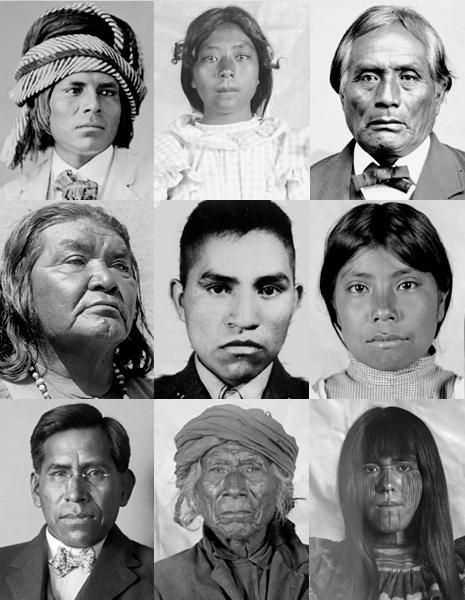
\includegraphics[width=0.2\textwidth]{Pima.jpeg}
        };
        \node[above=-3.5cm, left=0.5cm,font=\fontsize{5pt}{5pt}\selectfont] at (current page.0)  {Extraída desde Wikipedia.};
    \end{tikzpicture}
\end{frame}

%%%%%%%%%%%%%%%%
\end{document}